\begin{figure}[hp]
    \centering
    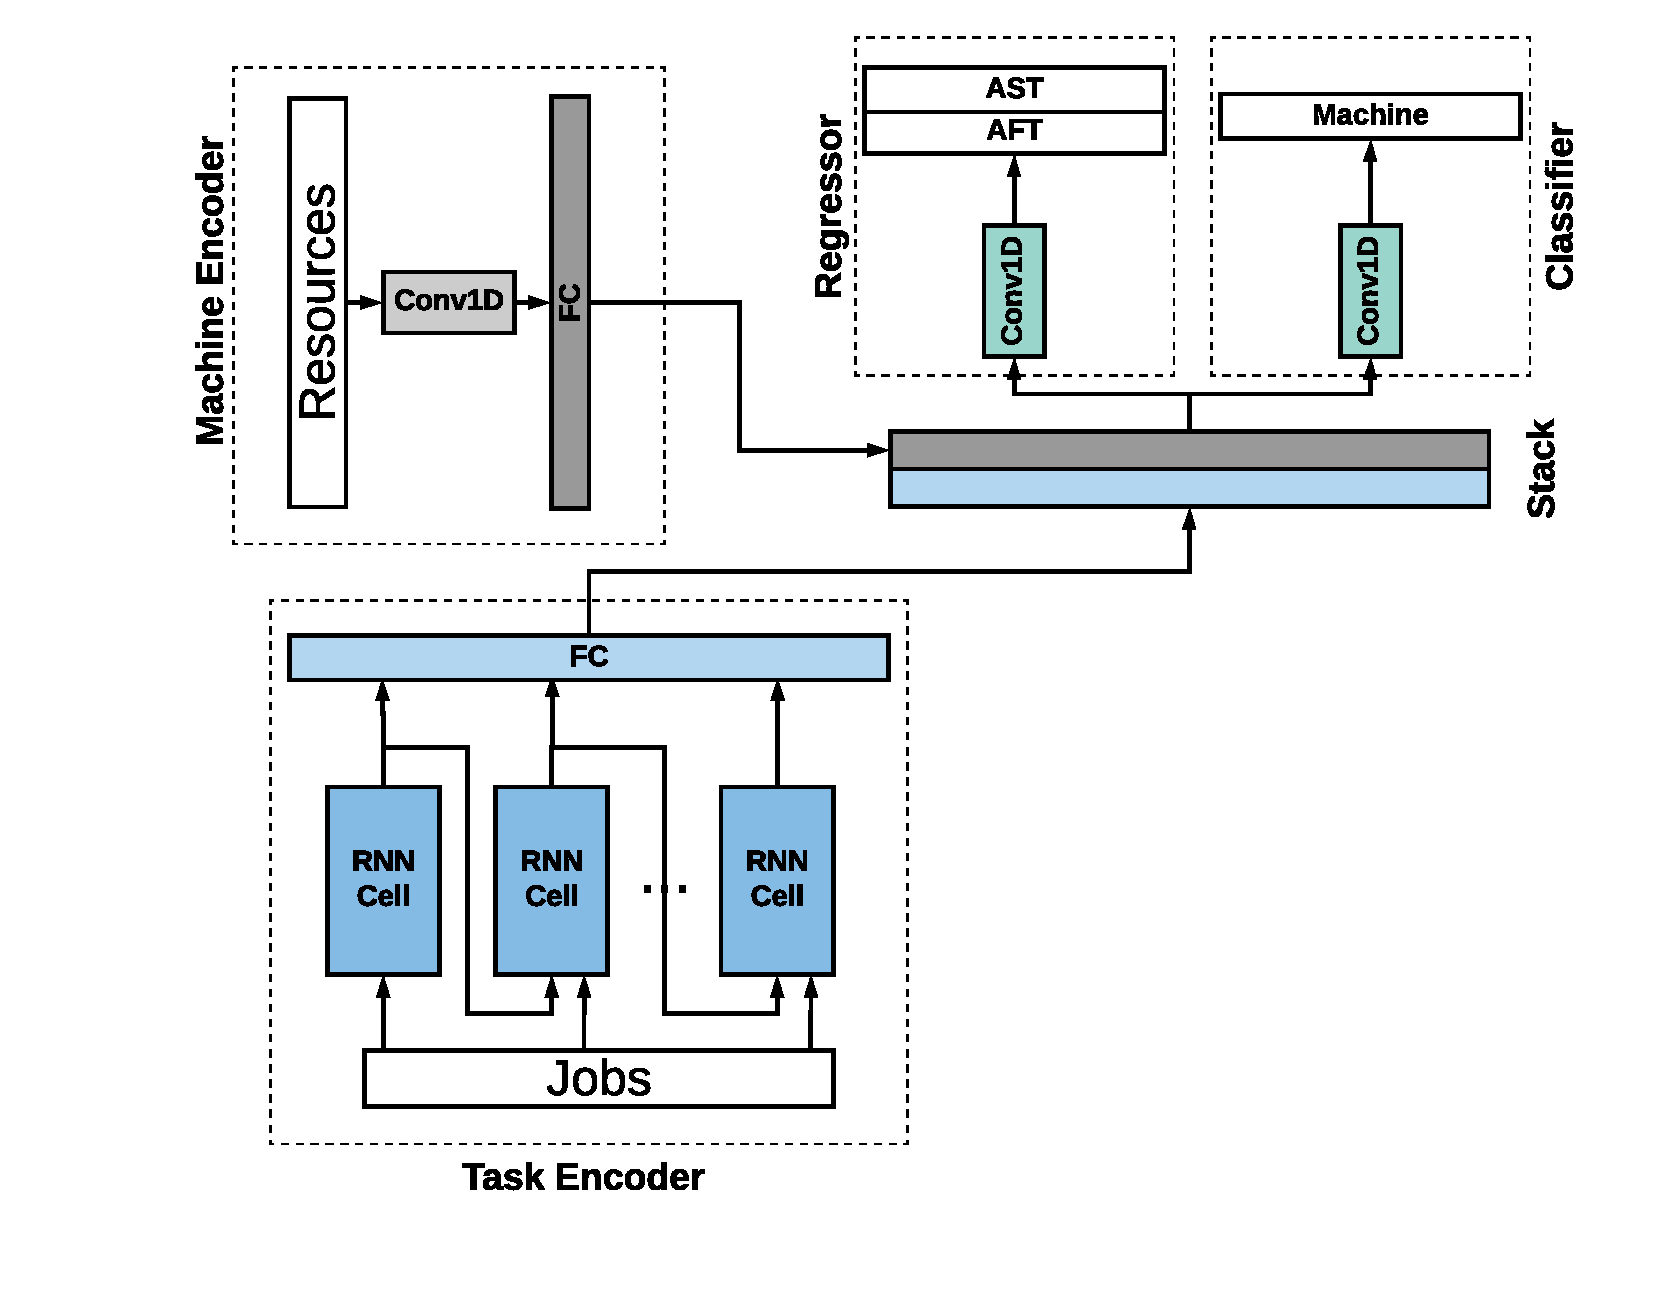
\includegraphics[width=0.45\textwidth]{diagrams/sched_nn}
    \caption{The architecture of the proposed neural network (DeepSched) for distributed heterogeneous systems scheduling.}
    \label{fig:nn}
\end{figure}

\subsection{Motivation}
Heterogeneous task scheduling is a relatively new concept, which lacks developers support. It's an active area of research, where many techniques are being developed through time. Being able to achieve the best possible performance on the given tasks, while keeping good utilization of resources is a tedious problem in heterogeneous systems. Aside from being accurate, the scheduling methods have to be fast in its execution, also they should not consume the system resources. 

Heterogeneous scheduling methods are very computationally expensive. However, neural networks are relatively fast in inference and research is being conducted on optimizing inference even more. So, if a neural network can approximate the performance of current scheduling method, it can replace this method in production. 

We study the ability of neural networks to approximate some heuristic methods and explore its accuracy and execution time against both heuristic and approximated methods.

\subsection{Formulation}
First, let us specify the main target of this work. As the task scheduling in heterogeneous distributed system is a vast field with lots of settings and algorithms \cite{inbook}, we choose our scheduling setting to be local and static. The goal of this work is to explore the ability of neural networks to approximate the performance of some well-established scheduling algorithms. In our setting, the algorithms are provided a list of tasks, each has its own execution time on different machines and a set of heterogeneous machines, on which the tasks are executed. We compare the results neural networks to some other heuristic and approximate methods.

Although, we choose local static scheduling, we assume that the neural approximation methods can work in other settings as well.

\subsection{Baseline}
Two baseline methods are considered. We choose \emph{Heterogeneous Earliest Finish Time} (HEFT) \cite{993206} to be our heuristic baseline, as it's one of the widely-used scheduling algorithms in heterogeneous systems. Also, genetic algorithms \cite{article2} is provided as a baseline for approximate methods. \\

\subsubsection{Heterogeneous Earliest Time First (HEFT)}
HEFT \cite{993206} is an old and well-established algorithm for scheduling in heterogeneous systems. It has been used as a baseline in research due to its near-optimal results. Basically, it's a greedy algorithm that chooses some process to run on some machine, if the former has the earliest finish time, with consideration of the special nature of the heterogeneous system. However, HEFT isn't practical for real-world systems, as the finish time of a process isn't usually known in advance. Also, the greedy nature of the HEFT scheduler makes it prone to failure in complex situations. \\

\subsubsection{Genetic Algorithms}
Genetic algorithms \cite{article2} have proven to be very efficient in solving some of the hardest optimization problem. Previous work on the use of genetic algorithms in task scheduling \cite{article2} is adapted to the heterogeneous setting by adding parameters for execution time of different tasks on different machines.

The targeted \emph{fitness function} is the average waiting time $W_t$ for all tasks. The fitness function for a specific schedule \emph{S} is given by:
\begin{equation}
\mathcal Fitness(S) = \frac{\sum_{i=1}^{N} W_{ti}}{N} \label{eq:ga}
\end{equation}
where \emph{N} is the number of tasks in the schedule, $W_t$ is the waiting time for a specific task.

\subsection{Neural Networks (Deep Learning)}
The main novel idea of this work is the use of \emph{neural networks} for the scheduling problem. Neural Networks are known to be very good at learning representations and function approximation. In this work, we propose an architecture that can be used to reach a good approximated solution for the scheduling problem. \emph{Offline Optimization} of neural networks is to be used, in order to be able to train the network on scheduling samples and then use the trained network to do inference. We avoid using \emph{online optimization}, used in some fields such as neural style transfer \cite{gatys2015neural}. This is because it's slow and we mainly care about execution time of the scheduling method.

Previous work tried to use neural networks to solve scheduling problem through \emph{Hopfield Nets} \cite{sathasivam2008logic} and \emph{Inhibitor Neurons} \cite{article3}. However, we try to make use of the recent advances in \emph{Deep Learning} to redefine the scheduling problem and solve it. 

As mentioned, The provided input is a list of tasks with its information and a set of machines. We want the network to learn an implicit representation of the given tasks and machines. Then, the network learn the mapping between the learned representation and the desired schedule. In other words, the target of the network is to take two input list of information of both tasks and machines and then output for each task, the machine to be executed on, the actual start time and the actual finish time. \\
    
\subsubsection{Architecture}
Our architecture consists of two encoders and one decoder, as shown in Fig.\ref{fig:nn}. \\
The first encoder is a fully convolutional network of \emph{1D} convolutional layers, to which is machines specifications are passed. This encoder learns a representation for the machines to be able to use it later in producing the outputs.

The second encoder is an \emph{Recurrent Neural Network} (RNN) \cite{chung2014empirical}, to which the tasks are passed one by one ordered by the arrival time. This network learns a representation of the tasks preserving the arrival order. RNN is chosen due to its proven effectiveness in dealing with sequential data, as they can learn complex temporal information from time sequences.

The two representations are then stacked and passed to two modules. A classification module which states the machine on which a specific task is executed. A regression module that identifies the actual start time and the actual finish time. Mainly, the two modules consist of \emph{1D} convolutional layers. 

Basically, the classifier is used during inference to produce the required schedule by determining the required machine for each task. However, the regressor is used at training along with the classifier, in order to add extra constraints on the network training and to enhance the loss function. This helps the network to learn a good representation of the scheduling problem and its parameters, also prevents the network from making some implicit mistakes in scheduling such as having two tasks executing on the same machine during the same range of time. \\
    
\subsubsection{Objective Function}
The cost function defined for this architecture is a sum of two criteria. The two criteria are categorical cross entropy \emph{(CE)} on the predicted machine to run a specific job $M_p$ and mean square error \emph{(MSE)} on the predicted actual start time $AST_p$ and the predicted actual finish time $AFT_p$. So, it can be summarized as follows:
\begin{equation}
\mathcal Loss(L) = CE(M_p, M_t) + MSE(AT_p, AT_t) \label{eq:l}
\end{equation}
where $M_p$ is the predicted machine, $M_t$ is the ground truth machine, $AT_p$ is the predicted actual time range and $AT_t$ is the ground truth actual time range. \\

\subsubsection{Drawbacks}
The main drawback of the proposed solution is that we have to know the maximum number of machines and the maximum number of tasks to be able to define the network. These numbers are used to define the network and loss function dimensions. So, the network design has to force some static scenarios to work on. However, this can be the case in some situations such as simulation workflow in supercomputers, where the tasks, to be executed, are known before the simulation starts. So, our proposed method can be suitable for these scenarios, as it can provide static execution time for different input sizes.  